
\section{Evaluation}
\label{sec:evaluation}

To assess the solution quality of 3SAT on a quantum annealing platform, using the previously discussed method of encoding 3SAT problems, we ran several experiments on a D-Wave 2000Q system. Using ToughSAT\footnote{\url{https://toughsat.appspot.com/}} we generated 3SAT instances of various difficulty (i.e., with various values for $\alpha$). However, as discussed in Section~\ref{sec:preliminaries}, for $|\alpha - 4.2| \gg 0$ problem instances become very easy to solve. We observed that effect on the quantum annealer as well, since all of these instances were easily solved on the D-Wave machine. Thus, for the remainder of this section, we focus on hard instances (approximated by $\alpha = 4.2$) to assess solution quality in the interesting problem domain.

Experiments have shown that using the standard embedding tools delivered with the D-Wave platform, we can only reliably find a working embedding on the D-Wave 2000Q chip for 3SAT instances with at most $42$ clauses~\cite{adams1995hitchhikers}. To maintain $\alpha \approx 4.2$, the generated 3SAT instances contain $10$ different variables. We only assess solution quality for 3SAT instances that are satisfiable, but do not
provide this information to the solver.

\begin{figure}[t]
\centering
%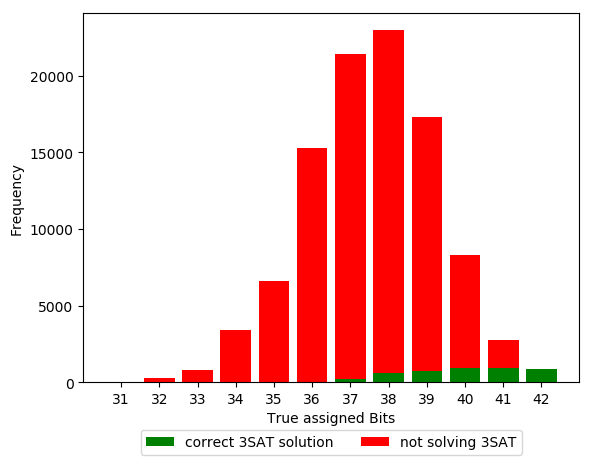
\includegraphics[width=.5\textwidth]{../material_2/Plots/42_4_2_def_engl_color_ohne_transform.png}%
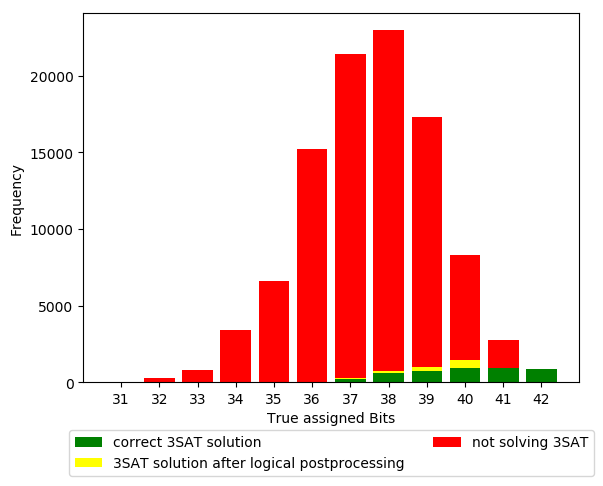
\includegraphics[width=.75\textwidth]{../material_2/Plots/42_4_2_def_engl_color_mit_transform.png}
\caption{Distribution of correct (green) and incorrect (red) answers returned by the quantum annealer \emph{without D-WAVE postprocessing}. Answers that can trivially be transformed into valid answers using logical postprocessing are marked in yellow. The plot shows 100,000 answers in total for 100 different hard 3SAT instances ($\alpha \approx 4.2$).}
\label{fig:distr-no-pp}
\end{figure}

Figure~\ref{fig:distr-no-pp} shows the result distribution of these runs on the D-Wave machine. On the x-axis, we sorted the returned results according to the bits that have been assigned the value $1$ or $\textit{True}$. As discussed in Section~\ref{sec:exp-setup} the optimal solution is supposed to set one bit for each clause, i.e., is supposed to contain 42 bits set to $\textit{True}$. However, as there are only 10 different variables, there theoretically exist answers that only set 10 bits but that still map to a complete and valid solution for the given 3SAT instance. From Figure~\ref{fig:distr-no-pp} we can see that some of these solution are found for bitcounts starting from 37 through 41. Interestingly, the complete range of answers gathered seems to follow a distribution centered around $37$ or $38$ and no answers with more than 42 bits are returned. This means that the constraint of never setting multiple bits per clause is fully respected in the evaluation of our QUBO matrix. It is important to note that although there are 5,283 correct solutions in total, these are only distributed across 24 of the 100 randomly generated problem instances. Thus,  most of them have not been solved at all.

Furthermore, we applied the logical postprocessing described in Section~\ref{sec:exp-setup} to the incorrect answers in Figure~\ref{fig:distr-no-pp}. However, it shows little improvement on the total amount of correct answers collected. We expect the postprocessing method delivered with the D-Wave software package to be more powerful as it runs local search along more axes of the solution space than the logical postprocessing does. So we ran the complete evaluation experiment again, only this time turning on the integrated postprocessing. The results are shown in Figure~\ref{fig:distr-yes-pp}.

\begin{figure}[t]
\centering
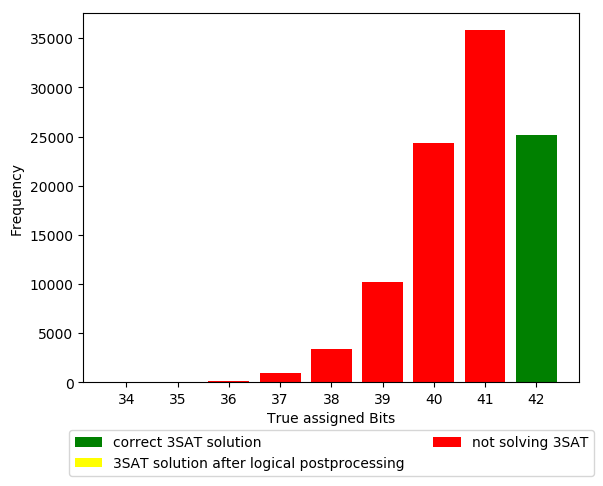
\includegraphics[width=.75\textwidth]{../material_2/Plots/42_4_2_opt_engl_color_mit_transform.png}
\caption{Distribution of correct (green) and incorrect (red) answers returned by the quantum annealer \emph{using D-WAVE postprocessing}. Answers that can trivially be transformed into valid answers using logical postprocessing are marked in yellow. The plot shows 100,000 answers in total for 100 different hard 3SAT instances ($\alpha \approx 4.2$).}
\label{fig:distr-yes-pp}
\end{figure}

We observed that the D-Wave postprocessing managed to optimize all correct but ``incomplete'' answers, mapping them to a solution with 42 bits assigned the value $\textit{True}$. Out of the 100,000 queries, this yielded 25,142 correct answers. Moreover, these correct answers span 99 of the 100 randomly generated 3SAT instances so that we consider the problem solved. Effectively, this shows that quantum annealing does suffer from a breakdown in performance at the point of the phase transition in the 3SAT problem. In comparison to the immense decrease in performance seen in classical solvers (cf. Section~\ref{sec:preliminaries}), a drop to around 25\% appears rather desirable, though. A quick example: To achieve a $1 - 10^{-12}$ confidence of returning the correct answer our experimental setup requires around $97$ queries. At a glance, that scaling factor with respect to problem difficulty is much better than what is observed for classical algorithms. It is important to note, however, that these experiments were performed for problem instances so small that their evaluation does not pose a challenge to classical processors at all, i.e., below the point of reasonable performance metrics. These results only proof relevant to practical applications if they scale with future versions of quantum annealing hardware that can tackle much larger problem instances.

So far, we have not discerned between different correct solutions. We were content as long as the algorithm returned but one. However, for the user it is interesting to know if he or she will receive the same solution with every answer or an even distribution across the complete solution space. Our experiments show that when a lot of correct solutions are found for a certain problem instance, there are cases where we can see a clear bias towards a specific solution variant. Figure~\ref{fig:distr-sols} shows the distributions of specific solutions. While some formulae seem to yield rather narrow distributions over the different possible answers, others definitely seem to have a bias towards certain solutions. However, the former also tend to have relatively smaller sample sizes as there are less solutions in total to consider. Further investigation could still reveal a distinctive distribution in these cases as well. Thus, we consider this behavior of the quantum annealer to be roughly in line with the findings of \cite{mandra2017exponentially}, who show an exponential bias in ground-state sampling of a quantum annealer.

\begin{figure}
\centering
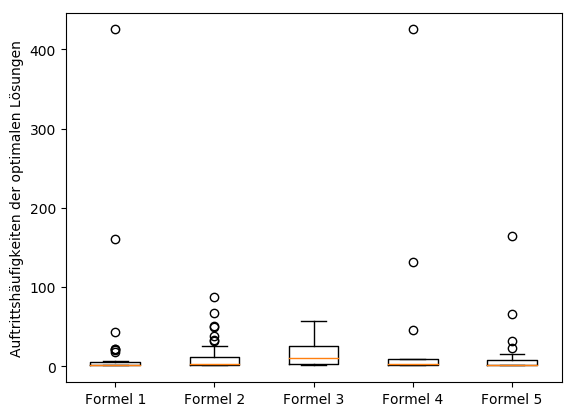
\includegraphics[width=.75\textwidth]{../material_2/25_clauses__4_2_def_MISBIAS.png}
\caption{Frequency of occurrence of different solutions for 5 formulae with many returned solutions. While most solutions are found once or just a few times, there are specific solutions that are found much more often.} \label{fig:distr-sols}
\end{figure}

%Lastly, we performed an additional experiment to check for the contingency of the presented results. As we have considered rather small problem instances (to the current limitations of the D-Wave chip) and a rather over-specified encoding of 3SAT (which allows for things like logical postprocessing to add benefit in the first place), we posed the question how much of solving these 3SAT instances actually requires an ``intelligent'' solving algorithm and how much part of the solution can be attributed to the environment. To examine this, we generated ``solutions'' to 3SAT instances using a random generator. We first considered a simple random generator that produced bitstrings of the same length as the D-Wave machine's answers. Figure~\ref{fig:distr-random} (left) shows the result for \emph{easy} 3SAT instances, i.e. $\alpha = 0.2$: Out of 100,000 queries for 100 different formulae, 19 returned answers represented a valid 3SAT solution. Interestingly, logical postprocessing was still able to yield another 2,425 solutions. When we increased the problem difficulty to the previously considered $\alpha = 4.2$, none of the randomly generated ``solutions'' were correct or could be postprocessed to be correct. Futhermore, we performed this test on another random generator which return bitstrings of the form $\{001, 010, 100\}^{42}$, i.e., solutions which are always correct at setting just one bit per 3SAT clause. While this allowed us to find more (i.e., 12,043) correct solutions in the easy instances  (cf. the right part of Figure~\ref{fig:distr-random}), we still id not generate a single correct solution among 10,000 for the transition point instances.

%\begin{figure}
%\centering
%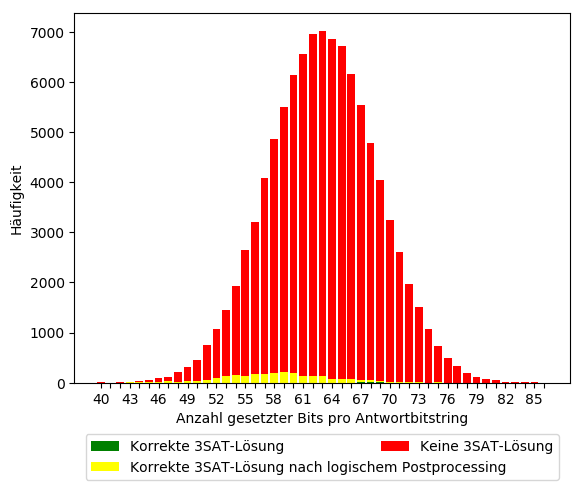
\includegraphics[width=.5\textwidth]{../material_2/42_clauses__0_2_def_RANDOM_color_transformed.png}%
%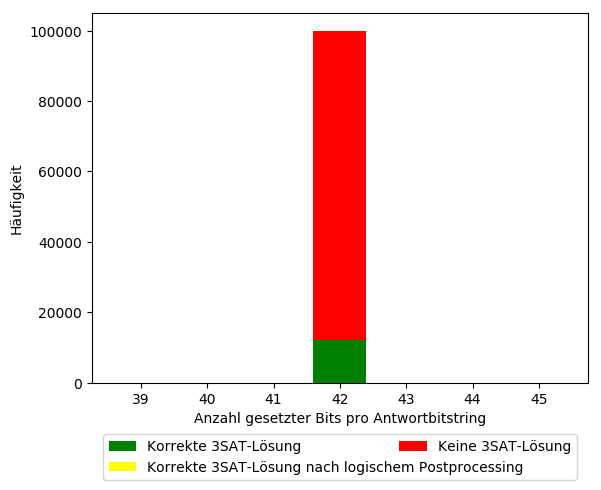
\includegraphics[width=.5\textwidth]{../material_2/42_clauses__0_2_def_RANDOM_CLEVER_color_transformed.png}
%\caption{Distribution of correct (green) and incorrect (red) answers returned by two different random generators. Answers that can trivially be transformed into valid answers using logical postprocessing are marked in yellow. Both plots shows 100,000 answers in total for 100 different hard 3SAT instances ($\alpha \approx 0.2$).} \label{fig:distr-random}
%\end{figure}


%Wie in Abschnitt \ref{krit:sat} dargelet wurde, gibt es bei 3SAT-Instanzen signifikante Unterschiede bezüglich der Schwierigkeit der Lösungsfindung. Das Verhältnis aus Anzahl der Klauseln zur Größe des Variablenpools , im Folgenden \emph{K/V-Verhältnis} genannt, bestimmt dabei die Schwierigkeit der Lösungsfindung. Unter Berücksichtigung dieses Sachverhalts werden im Folgenden zwei Versuchsreihen durchgeführt.
%\subsection{2. Versuchsreihe}
%In der 2. Versuchsreihe werden mit Hilfe des ToughSAT-Generators jeweils 100 zufällig generierte 3SAT-Formeln für die K/V-Verhältnisse 0.2, 4.2 sowie 8.4 erzeugt. Alle 3SAT-Formeln bestehen aus 42 Klauseln. Damit stehen zur Erzeugung der Formeln beim  K/V-Verhältnis von 0.2 insgesamt 210 Variablen, beim K/V-Verhältnis von 4.2 insgesamt 10 Variablen und beim K/V-Verhältnis von 8.4 insgesamt 5 Variablen zur Verfügung. Analog zur 1. Versuchsreihe werden hier alle 100 3SAT-Formeln der K/V-Verhältnisse 0.2 sowie 4.2 so gewählt, dass sie erfüllbar sind. Alle 3SAT-Formeln des K/V-Verhältnisses 8.4 sind so gewählt, dass sie nicht erfüllbar sind.
%\subsection{Versuchsdurchführung}
%Jedes 3SAT-Problem der 1. sowie der 2. Versuchsreihe wird zunächst auf ein WMIS-Problem reduziert (vgl. Kapitel \ref{red:sat:wmis}). Die Knoten des durch diese Reduktion entstanden Graphen \emph{$G_{SAT}$} werden mit dem  Gewicht 1 belegt, sämtliche Kanten mit dem Gewicht 4. Die Gewichte sind hier beliebig gewählt, jedoch so, dass das Kantengewicht jeder Kante größer ist als das Minimum der Gewichte der Knoten die diese Kante verbindet (vgl. Behauptung in Kapitel \ref{chap:wmis}). Anschließend werden aus diesem Graphen die linearen Gewichte der Ising-Energiefunktion berechnet (vgl. Gleichung \ref{red:6} bzw. \ref{red:7}). Nun kann das Problem dem DWAVE-Quantenannealer übergeben werden, der zunächst ein Embedding dieses Problems auf dem Chimera-Graphen bestimmt und anschließend durch Quantum Annealing eine Lösungs des Problems bestimmt. Für jede der in dieser Arbeit benutzten 3SAT-Formeln wird lediglich ein Embedding berechnet, welches dann für 1000 Annealingvorgänge benutzt wird. Man erhält also pro Formel insgesamt 1000 potentielle Lösungen.
%
%\todo{1 Colourful Pictures (6.11, 6.12, 6.15, 6.19 + Numbers from Tab. 6.4)}
%\todo{1 Explaining the colourful pictures}








